\documentclass[aspectratio=169]{beamer}
\usepackage{will_handley_beamer}
\usepackage{title_page}

% Commands
% --------
% - \arxiv{arxiv number}
% - \cols{width}{lh column}{rh column}
% -  \begin{fig(left|right)}[fractional width (e.g 0.6) ]{name of image}
%        content of other column
%    \end{fig(left|right)}

% Talk details
% ------------
\title{Nested sampling: powering next-generation Bayesian inference tools}
\subtitle{for cosmology, particle physics and beyond}
\date{14\textsuperscript{th} December 2022}

% Weds 14^th December 2022 : Day 2 - candidates present a research seminar to
% the department – this will be in hybrid format and recorded in order that
% members of the selection panel and other members of the department who are
% unable to be present in person to view the lectures.  Your seminar
% presentation should be of no more than 30 minutes' duration, with a further
% 5-10 minutes allotted for questions and  discussion.  The audience will
% include colleagues from several Departments, therefore the first half of
% your presentation should be a broad introduction to your area of research
% and view to the future, and must be accessible to faculty across all
% research  disciplines. The second half of your presentation may be as
% technical  as you wish.

\begin{document}

\begin{frame}
    \titlepage
\end{frame}

\begin{frame}
    \frametitle{What is Nested Sampling?}
    \begin{itemize}
        \item Nested sampling is a radical, multi-purpose numerical tool.
        \item Given a (scalar) function $f$ with a vector of parameters $\theta$, it can be used for:
    \end{itemize}
    \vspace{-10pt}
    \begin{columns}[t]
        \column{0.3\textwidth}
        \begin{block}{Optimisation}
            \[\theta_\text{max} = \max_\theta{f(\theta)}\]
        \end{block}
        \column{0.3\textwidth}
        \begin{block}{Exploration}
            \vspace{-10pt}
            \[\text{draw/sample}\quad \theta\sim f\]
            \vspace{-15pt}
        \end{block}
        \column{0.3\textwidth}
        \begin{block}{Integration}
            \[\int f(\theta) dV \]
        \end{block}
    \end{columns}
    \begin{columns}[t]
        \column{0.33\textwidth}
        \centerline{\includegraphics[width=0.8\textwidth,page=13]{figures/himmelblau}}
        \column{0.33\textwidth}
        \centerline{\includegraphics[width=0.8\textwidth,page=15]{figures/himmelblau}}
        \column{0.33\textwidth}
        \centerline{\includegraphics[width=0.8\textwidth,page=14]{figures/himmelblau}}
    \end{columns}
\end{frame}

\begin{frame}
    \frametitle{General setting}
    \begin{itemize}
        \item Integration is a fundamental concept in physics, statistics and data science:
    \end{itemize}
    \begin{columns}
        \column{0.3\textwidth}
        \begin{block}{Partition functions}
            \vspace{-11pt}
            \[ Z(\beta) = \int e^{-\beta H(q,p)} dq dp \]
        \end{block}
        \column{0.3\textwidth}
        \begin{block}{Path integrals}
            \[ \Psi = \int e^{i S} \mathcal{D}x \]
        \end{block}
        \column{0.3\textwidth}
        \begin{block}{Bayesian marginals}
            \vspace{-11pt}
            \[ \mathcal{Z}(D) = \int \mathcal{L}(D|\theta) \pi(\theta) d\theta \]
        \end{block}
    \end{columns}
    \begin{columns}
        \column{0.6\textwidth}
        \begin{itemize}
            \item Need numerical tools if analytic solution unavailable.
            \item High-dimensional numerical integration is hard.
            \item Riemannian strategy estimates volumes geometrically:
                \[ \int f(x) d^nx \approx \sum_i f(x_i) \Delta V_i \sim \mathcal{O}(e^n) \]
            \item Curse of dimensionality $\Rightarrow$ exponential scaling.
            \item Nested sampling integrates \textbf{probabilistically}.
        \end{itemize}
        \column{0.4\textwidth}
        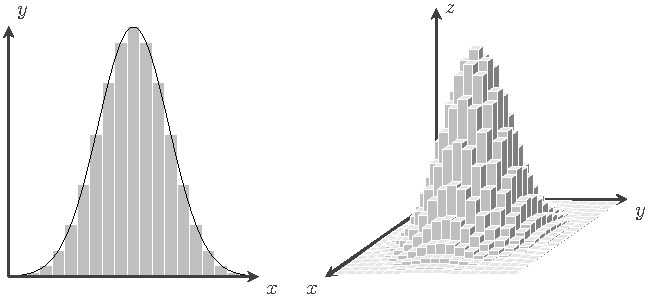
\includegraphics[width=\textwidth]{figures/integration.pdf}
    \end{columns}
\end{frame}

\begin{frame}
    \frametitle{The nested sampling meta-algorithm}
    \begin{columns}
        \column{0.5\textwidth}
        \begin{itemize}
            \item Start with $n$ random samples over the space.
            \item Delete outermost sample, and replace with a new random one at higher integrand value.
            \item The ``live points'' steadily contract around the peak(s) of the function.
            \item We can use this evolution to estimate volume \emph{probabilistically}.
            \item At each iteration, the contours contract by $\sim\frac{1}{n}\only<9->{\pm \frac{1}{n}}$ of their volume.
            \item This is an exponential contraction, so
                \[  \sum_i f(x_i) \Delta V_i, \qquad V_i = V_0 e^{-\only<9->{(}i\only<9->{\pm\sqrt{i})}/n} \]
%            \item Nested sampling: completely different way to scan.
%            \item Ensemble sampling compresses entire space$\to$peak(s).
%            \item Sequentially update a set $S$ of $n$ samples:
%                \begin{itemize}
%                    \item[$S_0$:]  Generate $n$ samples uniformly over the space (from a measure $\pi$). 
%
%                    \item[$S_{i+1}$:] Delete the lowest likelihood sample in $S_{i}$, and replace it with a new uniform sample with higher likelihood.
%                \end{itemize}
%            \item Requires one to be able to sample uniformly within a region, subject to a {\em hard constraint}:
%                \[\{\theta\sim \pi : \mathcal{L}(\theta)>\mathcal{L}_*. \}\]
%            \item This procedure optimises (multimodally), and can calculate the \C[3]{evidence}/integral of function \& \C[0]{posterior}/sample weights.
        \end{itemize}
        \column{0.5\textwidth}
        \includegraphics<1|handout:0>[width=\textwidth,page=1]{figures/himmelblau}%
        \includegraphics<2|handout:0>[width=\textwidth,page=2]{figures/himmelblau}%
        \includegraphics<3|handout:0>[width=\textwidth,page=3]{figures/himmelblau}%
        \includegraphics<4          >[width=\textwidth,page=4]{figures/himmelblau}%
        \includegraphics<5|handout:0>[width=\textwidth,page=5]{figures/himmelblau}%
        \includegraphics<6|handout:0>[width=\textwidth,page=6]{figures/himmelblau}%
        \includegraphics<7|handout:0>[width=\textwidth,page=7]{figures/himmelblau}%
        \includegraphics<8-|handout:0>[width=\textwidth,page=8]{figures/himmelblau}%
    \end{columns}
\end{frame}

\begin{frame}
    \frametitle{The nested sampling meta-algorithm}
    \begin{columns}
        \column{0.5\textwidth}
        \begin{itemize}
            \item At the end, one is left with a set of discarded ``dead'' points.
            \item Nested sampling estimates the \textbf{density of states} and calculates partition functions
                \[Z(\beta) = \sum_i f(x_i)^\beta \Delta V_i\]
            \item The evolving ensemble of live points allows:
                \begin{itemize}
                    \item implementations to self-tune
                    \item exploration of multimodal functions
                    \item global and local optimisation
                \end{itemize}
            \item For this kind of numerical, generic, high-dimensional integration, it is the only game in town.
            %\item Interpreted as a Bayesian algorithm, it
            %    \begin{itemize}
            %        \item Computes the Bayesian evidence (model comparison)
            %        \item Produces (weighted) posterior samples (parameter estimation)
            %    \end{itemize}
        \end{itemize}
        \column{0.5\textwidth}
        \includegraphics[width=\textwidth,page=14]{figures/himmelblau}%
        %\includegraphics<1|handout:0>[width=\textwidth,page=14]{figures/himmelblau}%
        %\includegraphics<2          >[width=\textwidth,page=15]{figures/himmelblau}%
    \end{columns}
\end{frame}

\begin{frame}
  \frametitle{Sampling from a hard likelihood constraint} 
  \begin{quote}
    ``It is not the purpose of this introductory paper to develop the technology of navigation within such a volume. We merely note that exploring a hard-edged likelihood-constrained domain should prove to be neither more nor less demanding than exploring a likelihood-weighted space.''\\
   {\hfill --- John Skilling}
  \end{quote}
  \begin{itemize}
      \item A large fraction of the work in nested sampling to date has been in attempting to implement a hard-edged sampler in the nested sampling meta-algorithm.
      \item \url{https://projecteuclid.org/euclid.ba/1340370944}.
      \item There has also been much work beyond this (focus of this talk).
  \end{itemize}
\end{frame}

\begin{frame}
    \frametitle{Implementations of Nested Sampling \arxiv{2205.15570}(NatReview)}
    \begin{columns}[t]
        \column{0.3\textwidth}
        \texttt{MultiNest}~\arxiv{0809.3437}
        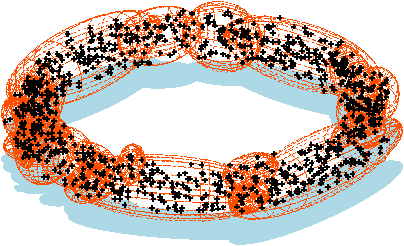
\includegraphics[width=\textwidth]{figures/multinest}
        \texttt{UltraNest}~\arxiv{2101.09604}
        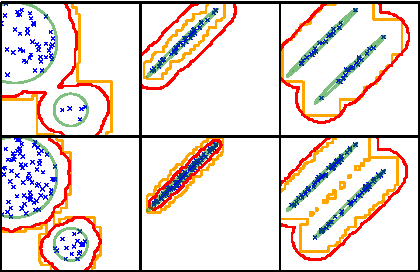
\includegraphics[width=\textwidth]{figures/radfriends}
        \column{0.3\textwidth}
        \texttt{PolyChord}~\arxiv{1506.00171}
        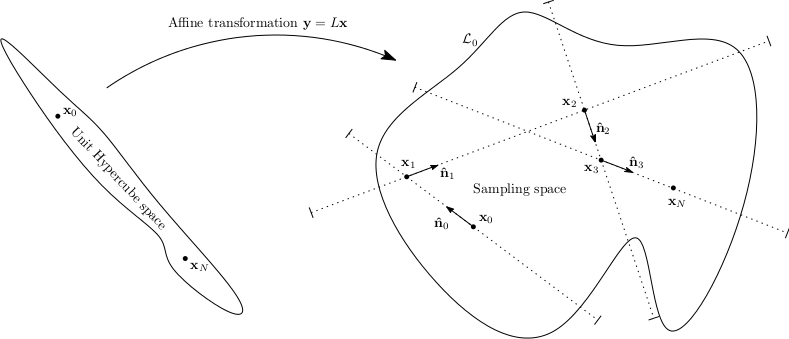
\includegraphics[width=\textwidth]{figures/polychord}
        \vfill
        \texttt{NeuralNest}~\arxiv{1903.10860}
        \begin{columns}
            \column{0.5\textwidth}
            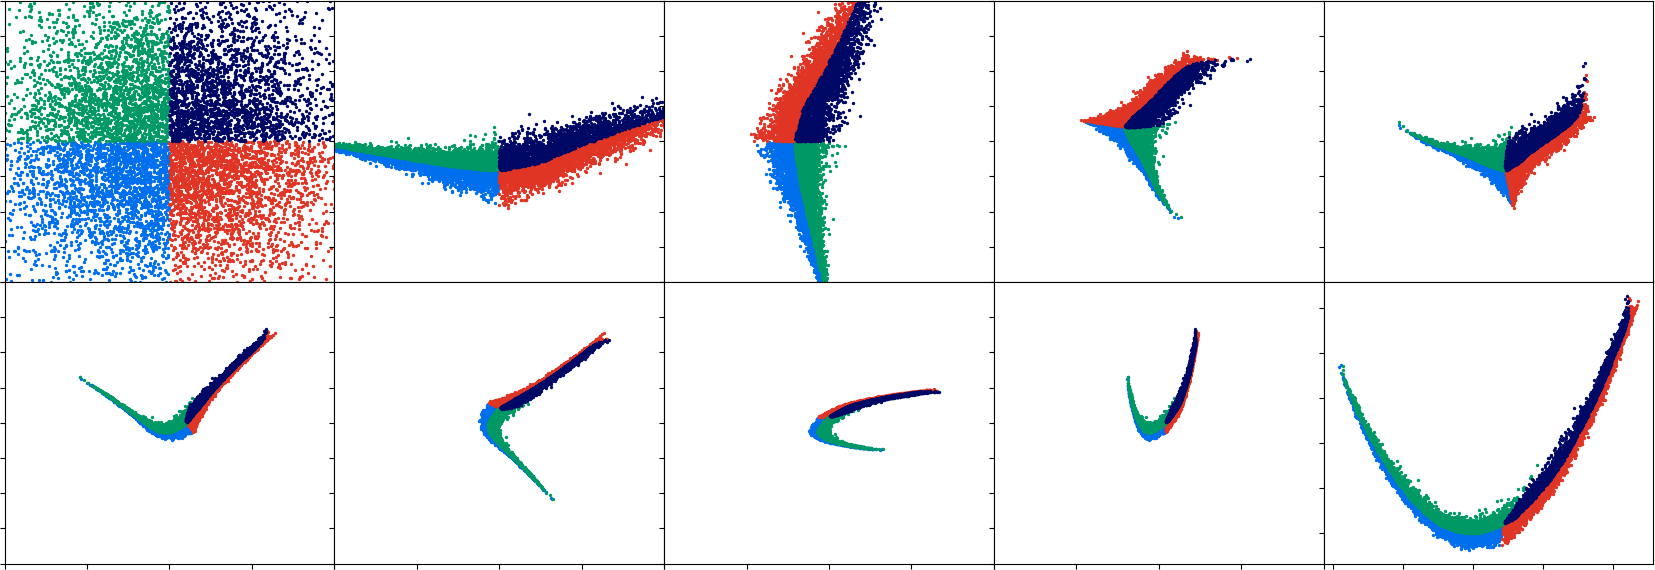
\includegraphics[width=\textwidth]{figures/rosenbrock_flow.png}
            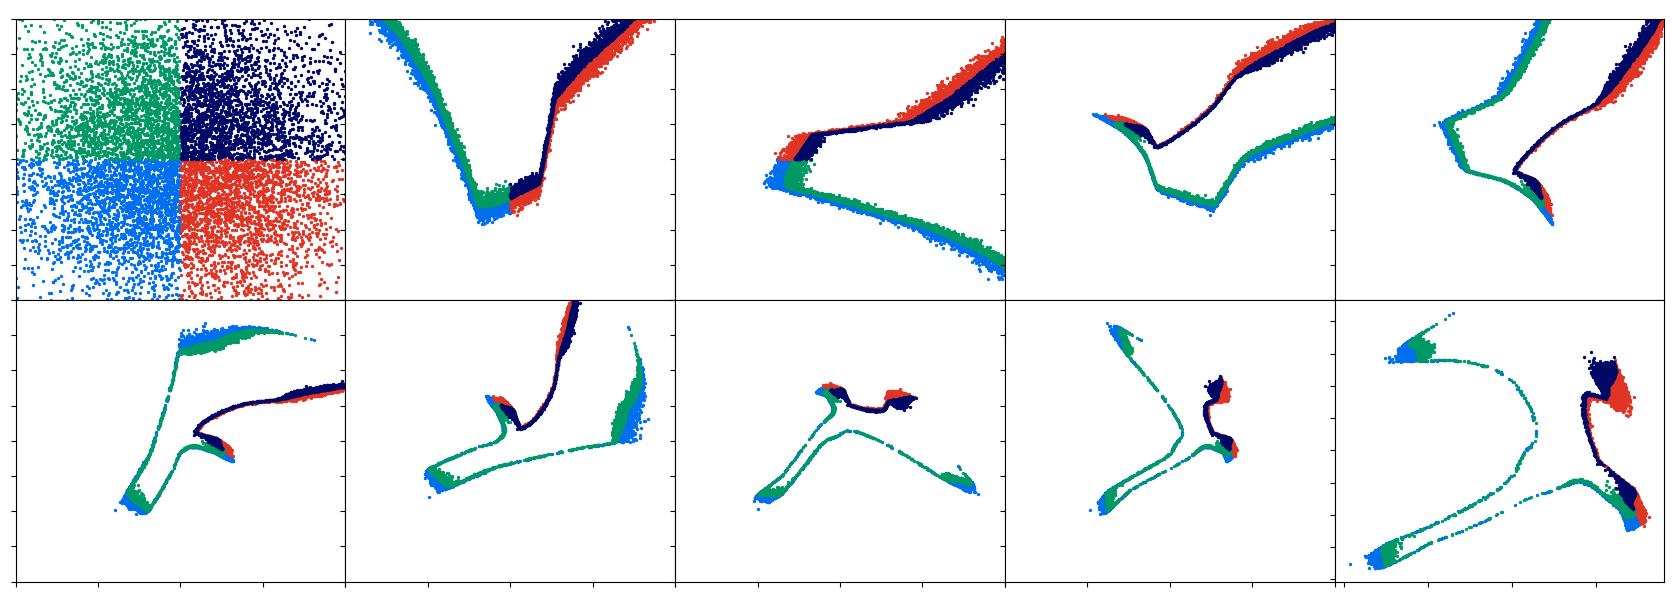
\includegraphics[width=\textwidth]{figures/himmelblau_flow.png}
            \column{0.5\textwidth}
            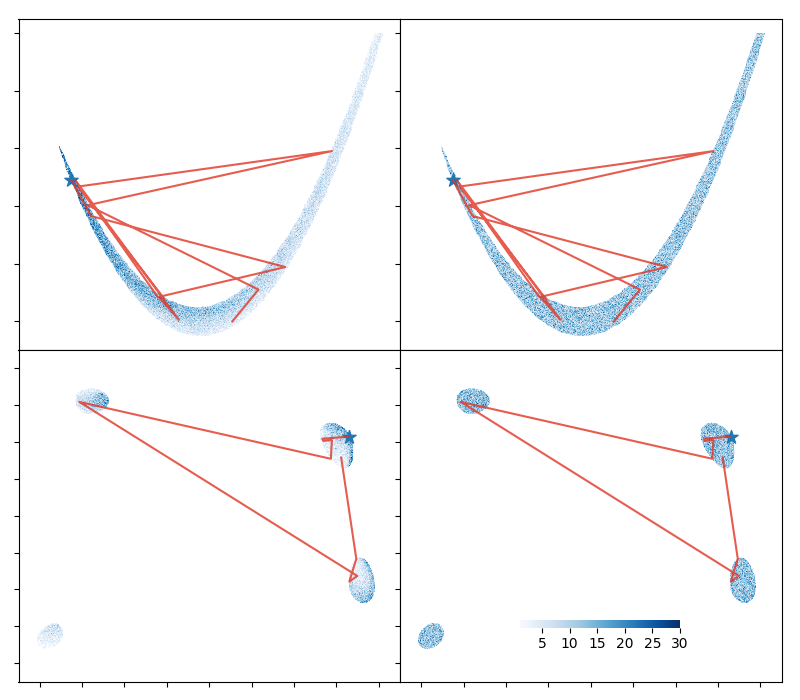
\includegraphics[width=\textwidth]{figures/chains.png}
        \end{columns}
        \texttt{dynesty}~\arxiv{1904.02180}
        \vfill
        \column{0.3\textwidth}
        \texttt{DNest}~\arxiv{1606.03757}
        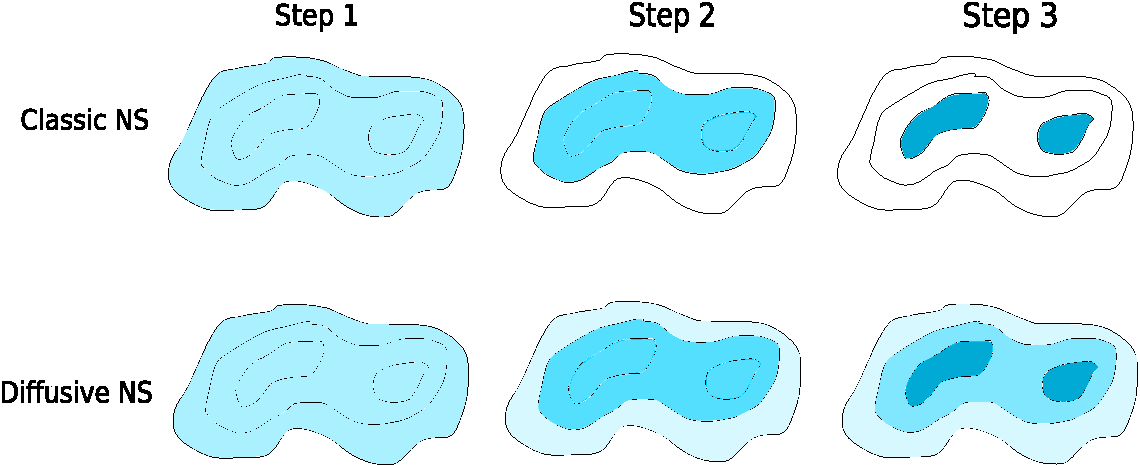
\includegraphics[width=\textwidth]{figures/dnest}
        \texttt{ProxNest}~\arxiv{2106.03646}
        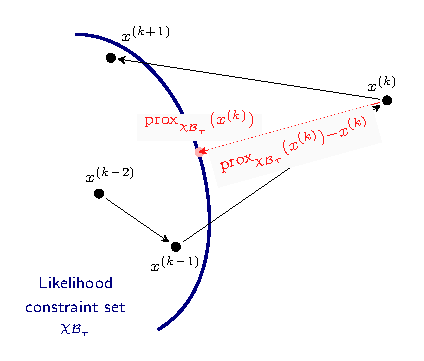
\includegraphics[width=\textwidth]{figures/proxnest_diagram}
        \vfill
    \end{columns}
\end{frame}

\begin{frame}
    \frametitle{Applications of nested sampling}
    \framesubtitle{Cosmology}
    \begin{columns}
        \column{0.55\textwidth}
        \begin{itemize}
            \item Battle-tested in Bayesian cosmology on
                \begin{itemize}
                    \item Parameter estimation: multimodal alternative to MCMC samplers.
                    \item Model comparison: using integration to compute the Bayesian evidence
                    \item Tension quantification: using deep tail sampling and suspiciousness computations.
                \end{itemize}
            \item Plays a critical role in major cosmology pipelines: Planck, DES, KiDS, BAO, SNe.
            \item The default $\Lambda$CDM cosmology is well-tuned to have Gaussian-like posteriors for CMB data. 
            \item Less true for alternative cosmologies/models and orthogonal datasets, so nested sampling crucial.
        \end{itemize}
        \column{0.45\textwidth}
        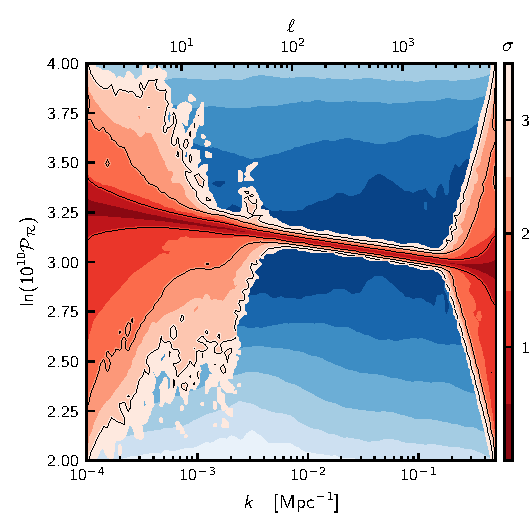
\includegraphics[width=0.49\textwidth]{figures/pps_both}
        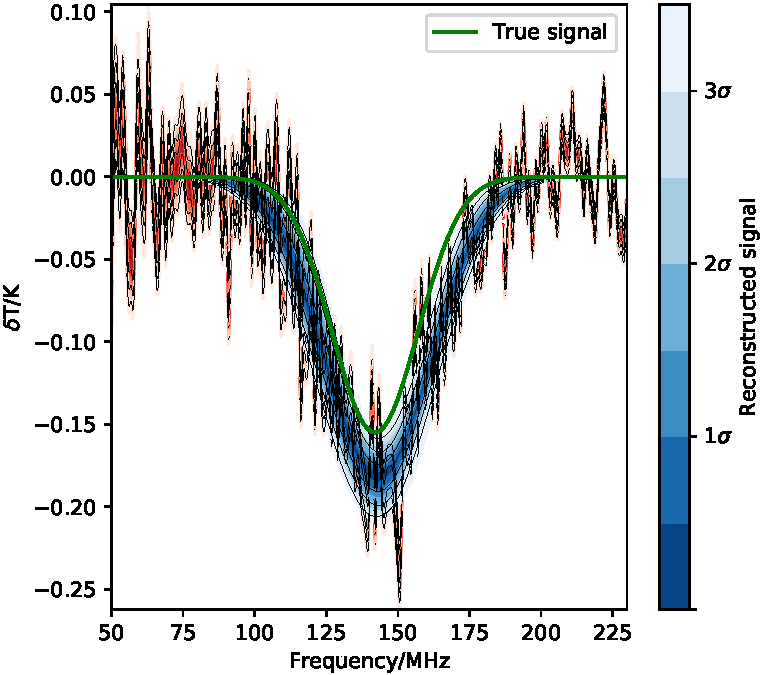
\includegraphics[width=0.49\textwidth]{figures/reach_fit-cropped.pdf}
        %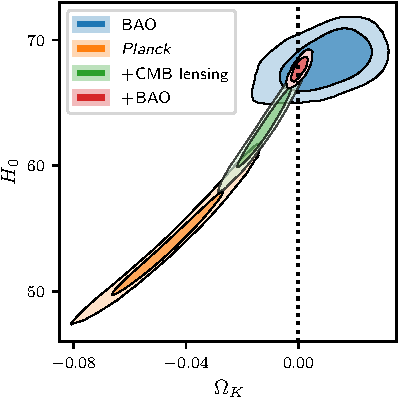
\includegraphics[width=0.49\textwidth]{figures/curvature_3}
        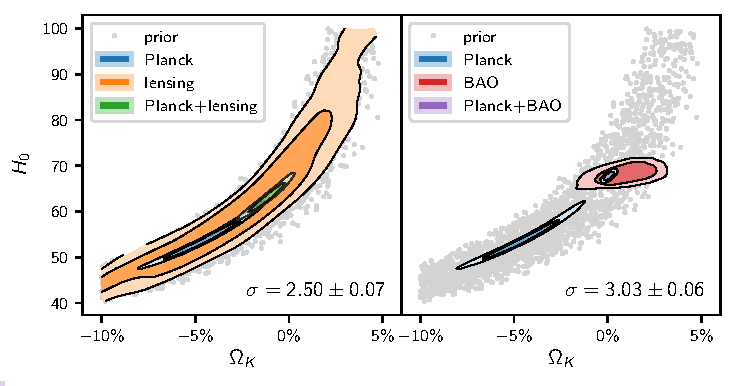
\includegraphics[width=\textwidth]{figures/omegak_H0_2.pdf}
    \end{columns}
\end{frame}

\begin{frame}
    \frametitle{Applications of nested sampling}
    \framesubtitle{Astrophysics}
    \begin{columns}
        \column{0.6\textwidth}
        \begin{itemize}
            \item In exoplanets~\arxiv{1806.00518}
                \begin{itemize}
                    \item Parameter estimation: determining properties of planets.
                    \item Model comparison: how many planets? Stellar modelling~\arxiv{2007.07278}.
                    \item exoplanet problems regularly have posterior phase transitions \arxiv{2102.03387}
                \end{itemize}
            \item In gravitational waves
                \begin{itemize}
                    \item Parameter estimation: Binary merger properties
                    \item Model comparison: Modified theories of gravity, selecting phenomenological parameterisations~\arxiv{1803.10210}
                    \item Likelihood reweighting: fast slow properties
                \end{itemize}
        \end{itemize}
        \column{0.4\textwidth}
        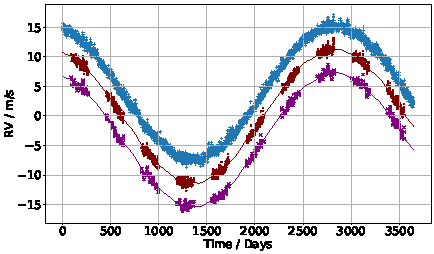
\includegraphics[width=\textwidth]{figures/rv_full.pdf}
        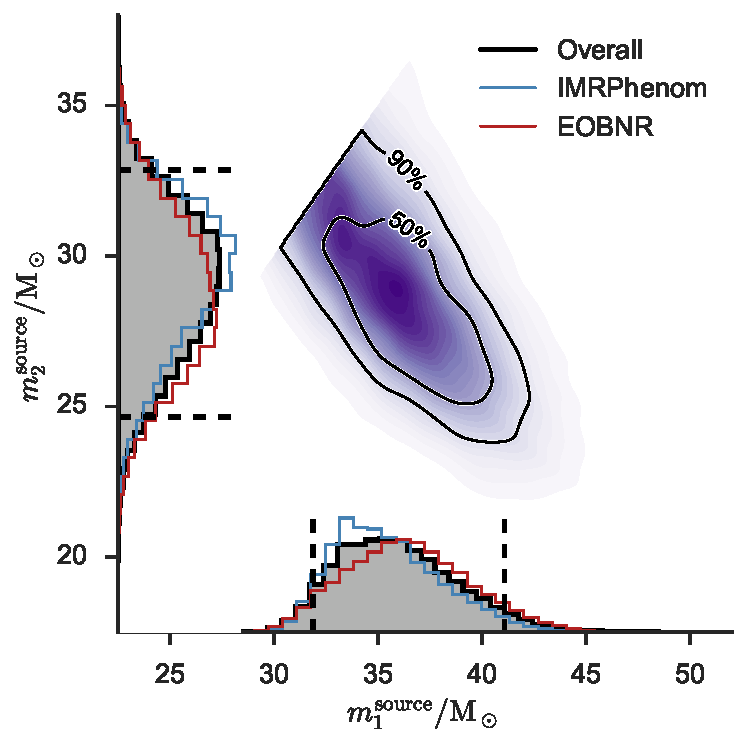
\includegraphics[width=0.49\textwidth]{figures/ligo_m1_m2.pdf}
        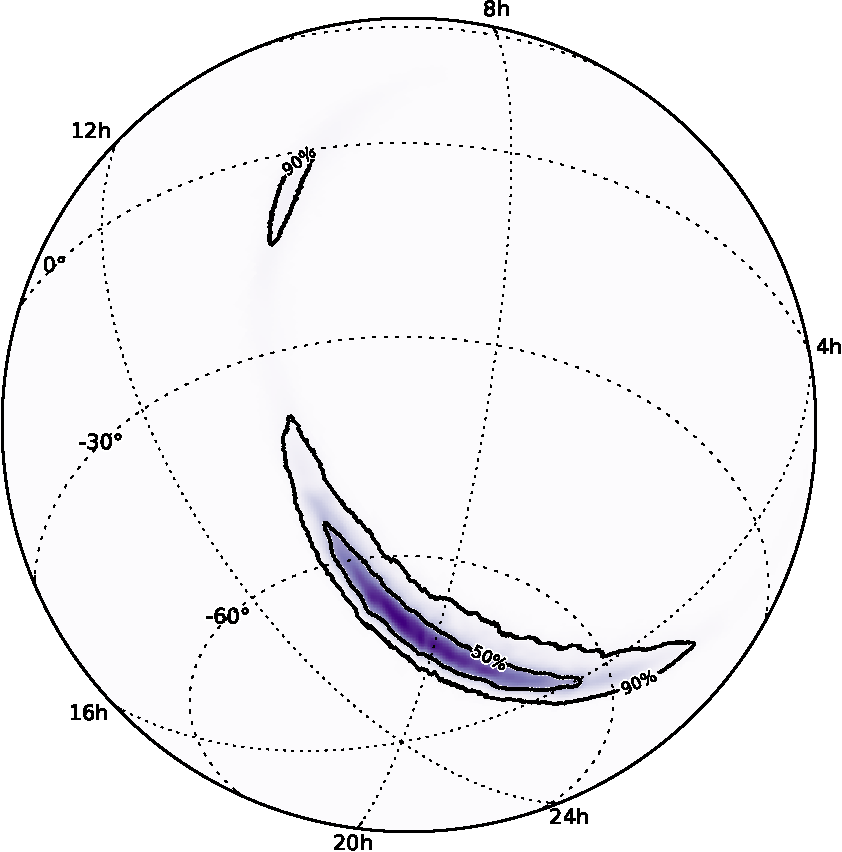
\includegraphics[width=0.49\textwidth]{figures/ligo_lambert-skymap.pdf}
    \end{columns}
\end{frame}

\begin{frame}
    \frametitle{Applications of nested sampling}
    \framesubtitle{Particle physics}
    \begin{columns}
        \column{0.56\textwidth}
        \begin{columns}
            \column{0.67\textwidth}
            \begin{itemize}
                \item Nested sampling for cross section computation/event generation
            \end{itemize}
            \column{0.3\textwidth}
            \[\sigma = \int_\Omega d\Phi |\mathcal{M}|^2.\]
        \end{columns}
        \begin{itemize}
            \item Nested sampling can explore the phase space $\Omega$ and compute integral blind with comparable efficiency to HAAG/RAMBO~\arxiv{2205.02030}.
            \item Bayesian sparse reconstruction~\arxiv{1809.04598} applied to bump hunting allows evidence-based detection of signals in phenomenological backgrounds~\arxiv{2211.10391}.
            \item Now applying to lattice field theory, and lattice gravity Lagrangians.
            \item Particle statistics: fast estimation of small $p$-values~\arxiv{2106.02056}(PRL).
        \end{itemize}
        \column{0.17\textwidth}
        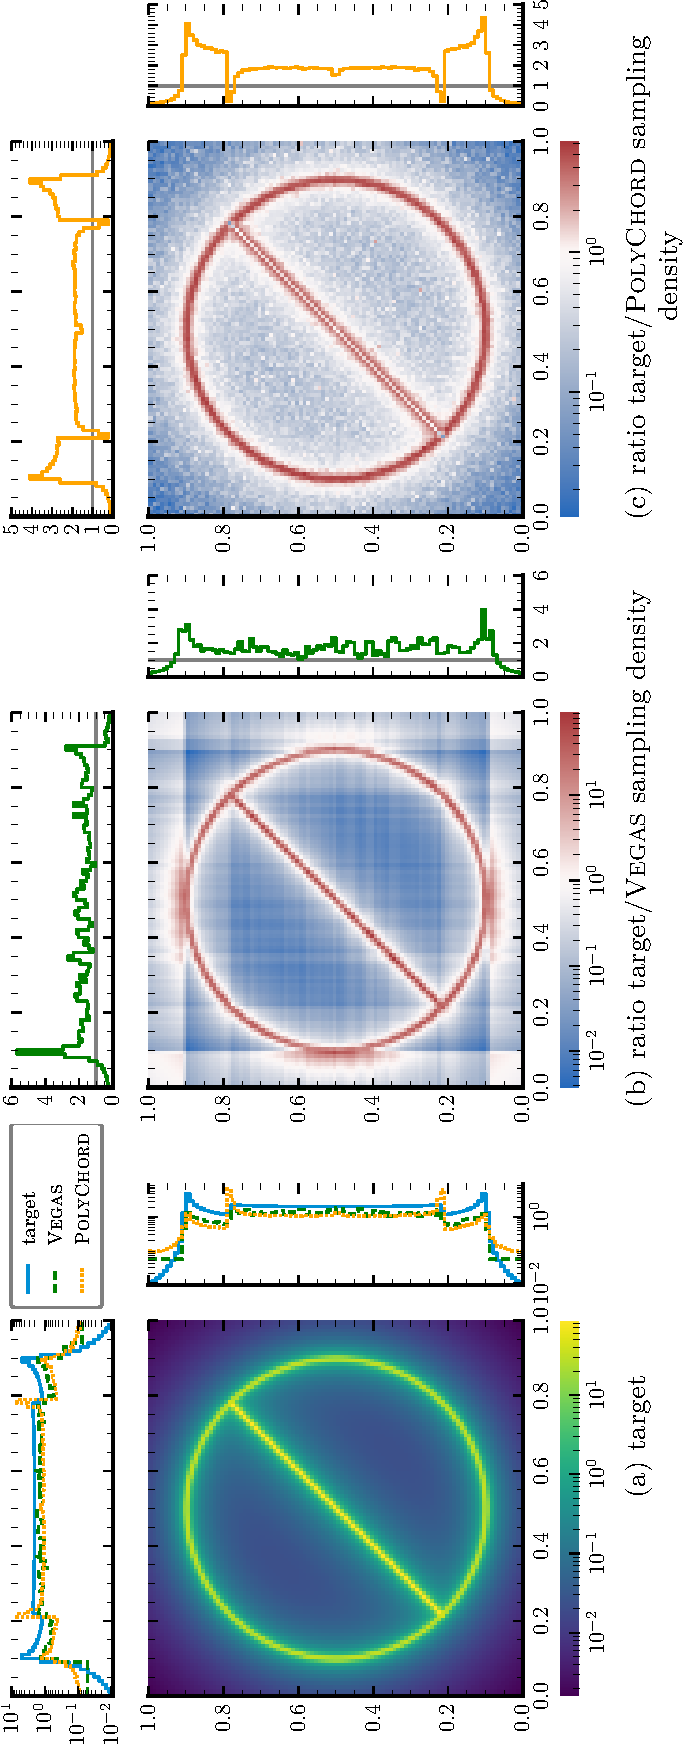
\includegraphics[width=\textwidth]{figures/phase_space_1-pdfjam-crop.pdf}
        \column{0.27\textwidth}
        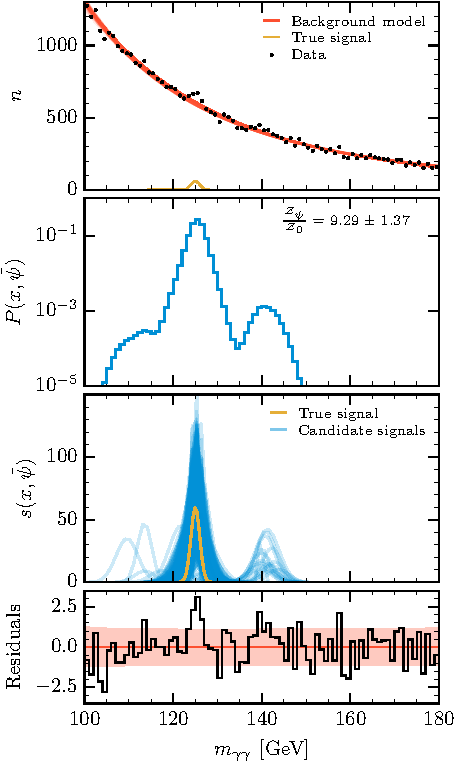
\includegraphics[width=\textwidth]{figures/psi_predict-crop.pdf}
    \end{columns}
\end{frame}

\begin{frame}
    \frametitle{Applications of nested sampling}
    \framesubtitle{Machine learning}
    \begin{columns}
        \column{0.62\textwidth}
        \begin{itemize}
            \item Machine learning requires:
                \begin{itemize}
                    \item Training to find weights
                    \item Choice of architecture/topology/hyperparameters
                \end{itemize}
            \item Bayesian NNs treat training as a model fitting problem
            \item Compute posterior of weights (parameter estimation), rather than optimisation (gradient descent)
            \item Use evidence to determine best architecture (model comparison), correlates with out-of-sample performance! 
            \item Solving the full ``shallow learning'' problem without compromise \arxiv{2004.12211}\arxiv{2211.10391}. 
            \item Promising work ongoing to extend this to transfer learning and deep nets.
        \end{itemize}
        \column{0.38\textwidth}
        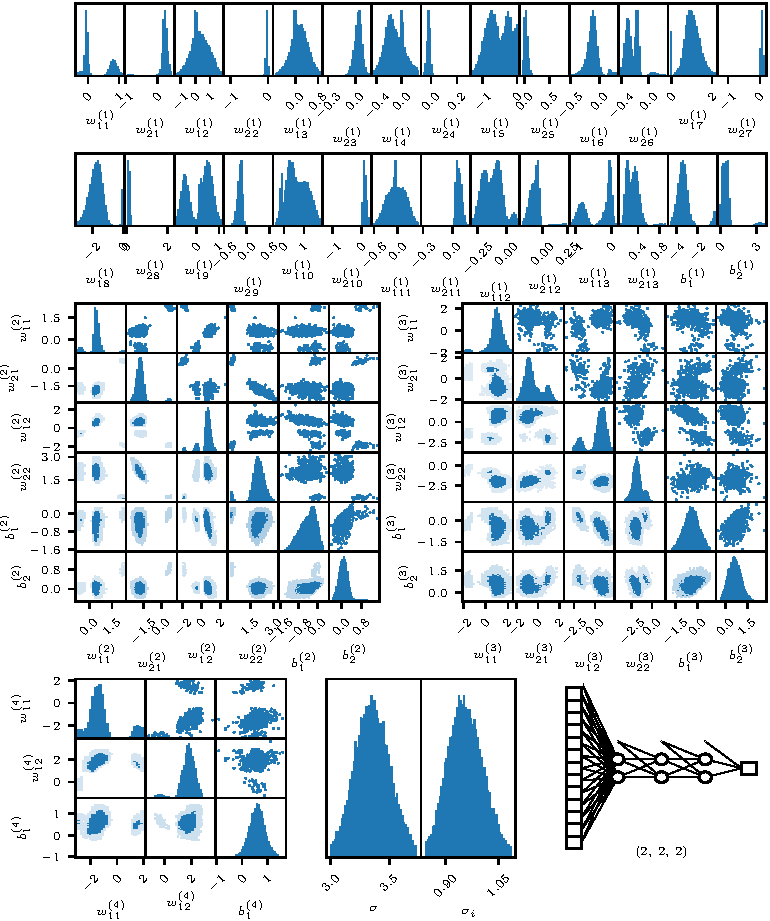
\includegraphics[width=\textwidth]{figures/nn_posterior-cropped.pdf}
    \end{columns}
\end{frame}

%\begin{frame}
%    \frametitle{Applications of nested sampling}
%    \framesubtitle{Statistics: fast estimation of small $p$-values~\arxiv{2106.02056}(PRL)}
%    \begin{columns}
%        \column{0.57\textwidth}
%        \begin{itemize}
%            \item Nested sampling for frequentist computation!?
%            \item $p$-value: $P(\lambda>\lambda^*|H_0)$ -- probability that test statistic $\lambda$ is at least as great as observed $\lambda^*$.
%            \item Computation of a tail probability from sampling distribution of $\lambda$ under $H_0$.
%            \item For gold-standard $5\sigma$, this is very expensive to simulate directly ($\sim10^9$ by definition).
%            \item Need insight/approximation to make efficient.
%            \item Nested sampling is tailor-made for this, just make switch: $X\leftrightarrow p$, $\mathcal{L}\leftrightarrow\lambda$, $\theta \leftrightarrow x$.
%            \item The only real conceptual shift is switching the integrator from parameter- to data-space.
%        \end{itemize}
%        \column{0.43\textwidth}
%        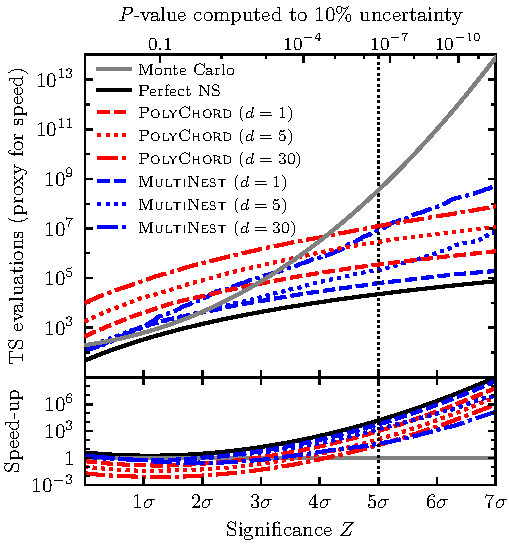
\includegraphics[width=\textwidth]{figures/pvalue.pdf}
%    \end{columns}
%\end{frame}

\begin{frame}
    \frametitle{Applications of nested sampling}
    \framesubtitle{and beyond\ldots}
    \begin{columns}
        \column{0.6\textwidth}
        \begin{itemize}
            \item Techniques have been spun-out (PolyChord Ltd) to:
            \item Protein folding
                \begin{itemize}
                    \item Navigating free energy surface.
                    \item Computing misfolds.
                    \item Thermal motion.
                \end{itemize}
            \item Nuclear fusion reactor optimisation
                \begin{itemize}
                    \item multi-objective.
                    \item uncertainty propagation.
                \end{itemize}
            \item Telecoms \& DSTL research (MIDAS)
                \begin{itemize}
                    \item Optimising placement of transmitters/sensors.
                    \item Maximum information data acquisition strategies.
                \end{itemize}
        \end{itemize}
        \includegraphics<1->[width=0.082\textwidth]{figures/headshots/watkinson-headshot.jpg}%
        \includegraphics<1->[width=0.082\textwidth]{figures/headshots/mason-headshot.jpg}%
        \includegraphics<1->[width=0.082\textwidth]{figures/headshots/formanek-headshot.jpg}%
        \includegraphics<1->[width=0.082\textwidth]{figures/headshots/mcaloone-headshot.jpg}%
        \includegraphics<1->[width=0.082\textwidth]{figures/headshots/stenczel-headshot.jpg}%
        \includegraphics<1->[width=0.082\textwidth]{figures/headshots/yallup-headshot.jpg}%
        \includegraphics<1->[width=0.082\textwidth]{figures/headshots/bex-headshot.jpg}%
        \includegraphics<1->[width=0.082\textwidth]{figures/headshots/claireburke-headshot.jpg}%
        \includegraphics<1->[width=0.082\textwidth]{figures/headshots/hobson-headshot.jpg}%
        \includegraphics<1->[width=0.082\textwidth]{figures/headshots/lasenby-headshot.jpg}%
        \includegraphics<1->[width=0.082\textwidth]{figures/headshots/mhandley-headshot.jpg}%
        \includegraphics<1->[width=0.082\textwidth]{figures/headshots/whandley-headshot.jpg}%
        \column{0.4\textwidth}
        \includegraphics<1|handout:0>[width=\textwidth]{figures/protein_1.png}%
        \includegraphics<2          >[width=\textwidth]{figures/protein_2.png}%
        \includegraphics<3|handout:0>[width=\textwidth]{figures/protein_3.png}%
        \includegraphics<4|handout:0>[width=\textwidth]{figures/lcoe.png}%
        %\includegraphics<5|handout:0>[width=\textwidth]{figures/tdoa-cropped-1-crop.pdf}%
        %\includegraphics<6|handout:0>[width=\textwidth]{figures/tdoa-cropped-2-crop.pdf}%
        %\includegraphics<7|handout:0>[width=\textwidth]{figures/tdoa-cropped-3-crop.pdf}%
        \includegraphics<5|handout:0>[width=\textwidth]{figures/DKL_contour-cropped-crop.pdf}%
        \includegraphics<6|handout:0>[width=\textwidth]{figures/mean_DKL_optimise-3-crop.pdf}%
        \includegraphics<7|handout:0>[width=\textwidth]{figures/mean_DKL_optimise-4-crop.pdf}%
        \includegraphics<8|handout:0>[width=\textwidth]{figures/mean_DKL_optimise-5-crop.pdf}%
    \end{columns}
\end{frame}

\begin{frame}
    \frametitle{Beyond the meta-algorithm}
    \begin{columns}
        \column{0.5\textwidth}
        \begin{itemize}
            \item Dynamic nested sampling~\arxiv{1704.03459}
            \item Unwoven nested sampling~\arxiv{1703.09701}
            \item Accelerated nested sampling~\arxiv{2212.01760}
            \item Precision nested sampling~\arxiv{2006.03371}
            \item Multiobjective nested sampling
            \item Nested sampling with gradients?
            \item Reversible nested sampling?
            \item Transdimensional nested sampling?
            \item postprocessing: \texttt{anesthetic}~\arxiv{1905.04768}
            \item crosschecking: \texttt{nestcheck}~\arxiv{1804.06406}
        \end{itemize}
        \column{0.5\textwidth}
        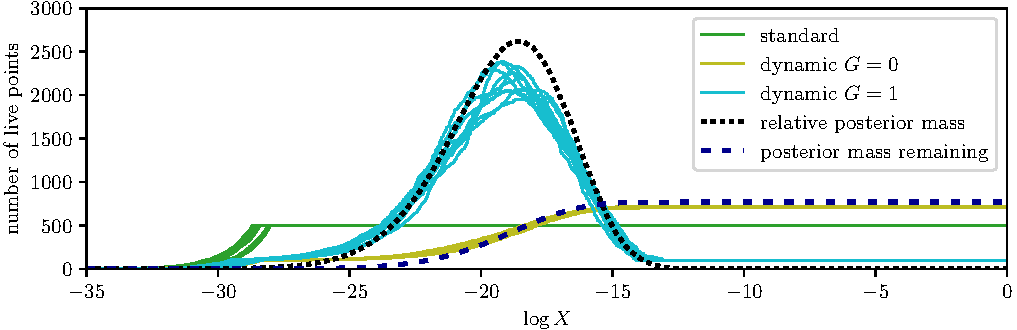
\includegraphics[width=\textwidth]{figures/dynesty.pdf}
        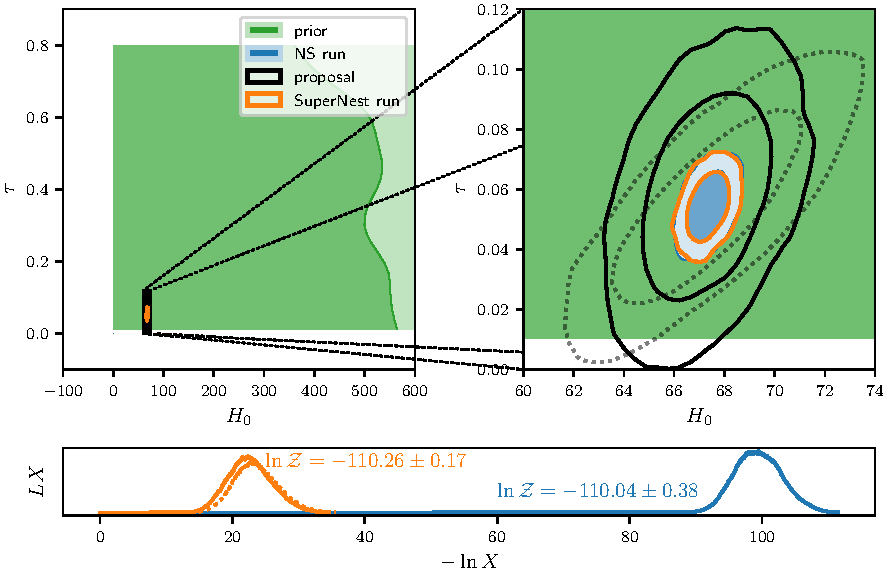
\includegraphics[width=\textwidth]{figures/supernest.pdf}
    \end{columns}
\end{frame}

\begin{frame}
    \frametitle{REACH: Global 21cm cosmology \arxiv{2210.07409}(NatAstro)}
    \begin{columns}
        \column{0.65\textwidth}
        \vspace{-10pt}
        \begin{itemize}
            \item Imaging the universal dark ages using CMB backlight.
            \item $21\text{cm}$ hyperfine line emission from neutral hydrogen.
            \item Global experiments measure monopole across frequency.
            \item Challenge: science hidden in foregrounds $\sim 10^4\times$signal.
            \item Lead data analysis team (REACH first light in January)
            \item Nested sampling woven in from the ground up (calibrator, beam modelling, signal fitting, likelihood selection).
            \item All treated as parameterised model comparison problems.
        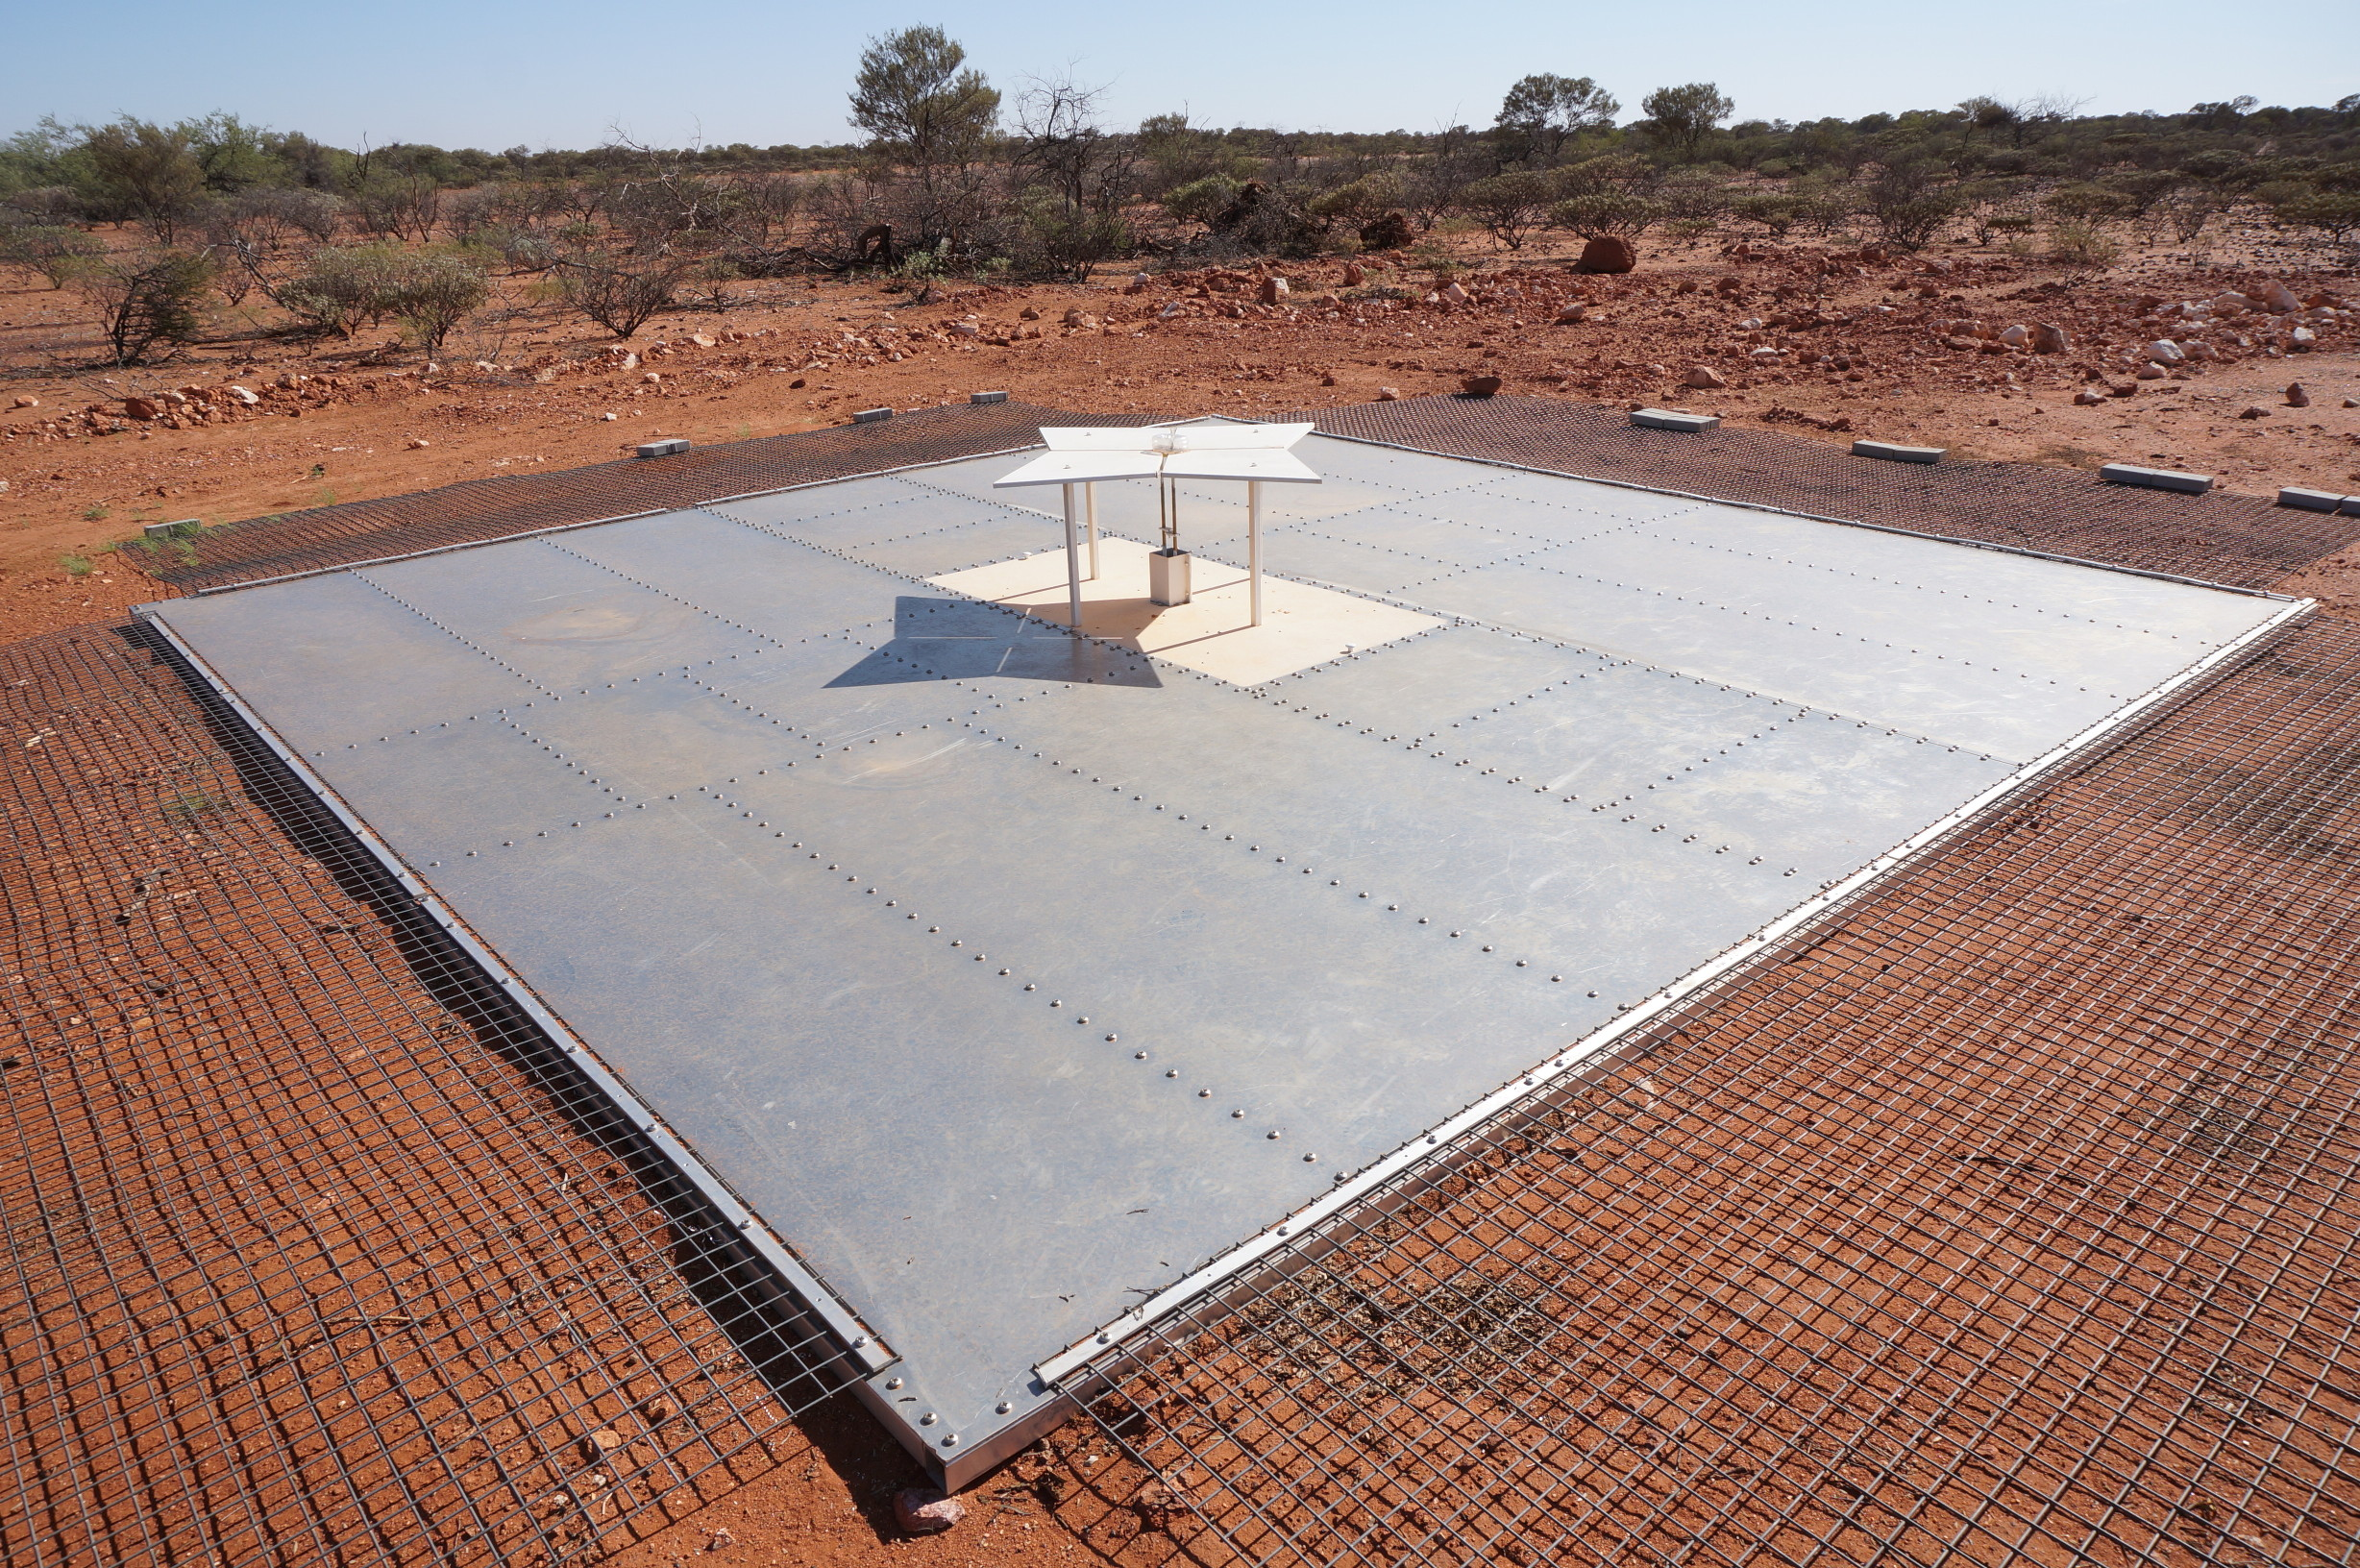
\includegraphics[height=0.3\textwidth]{figures/EDGES_antenna}
        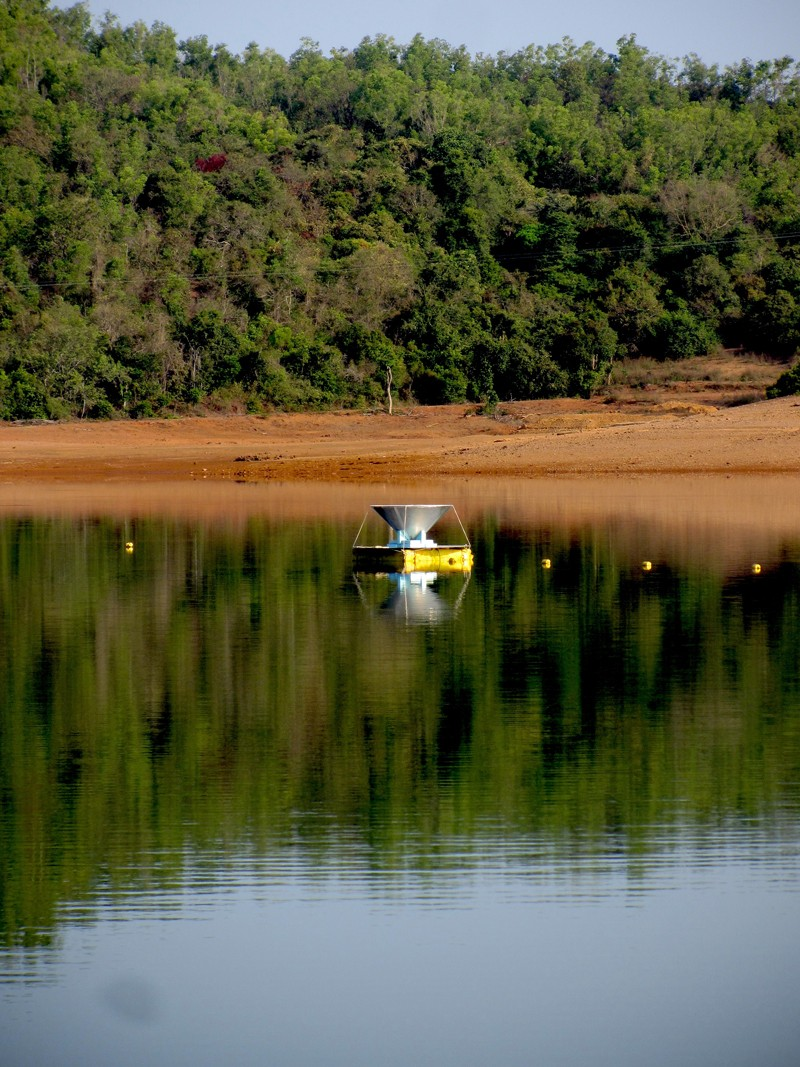
\includegraphics[height=0.3\textwidth]{figures/SARAS}
        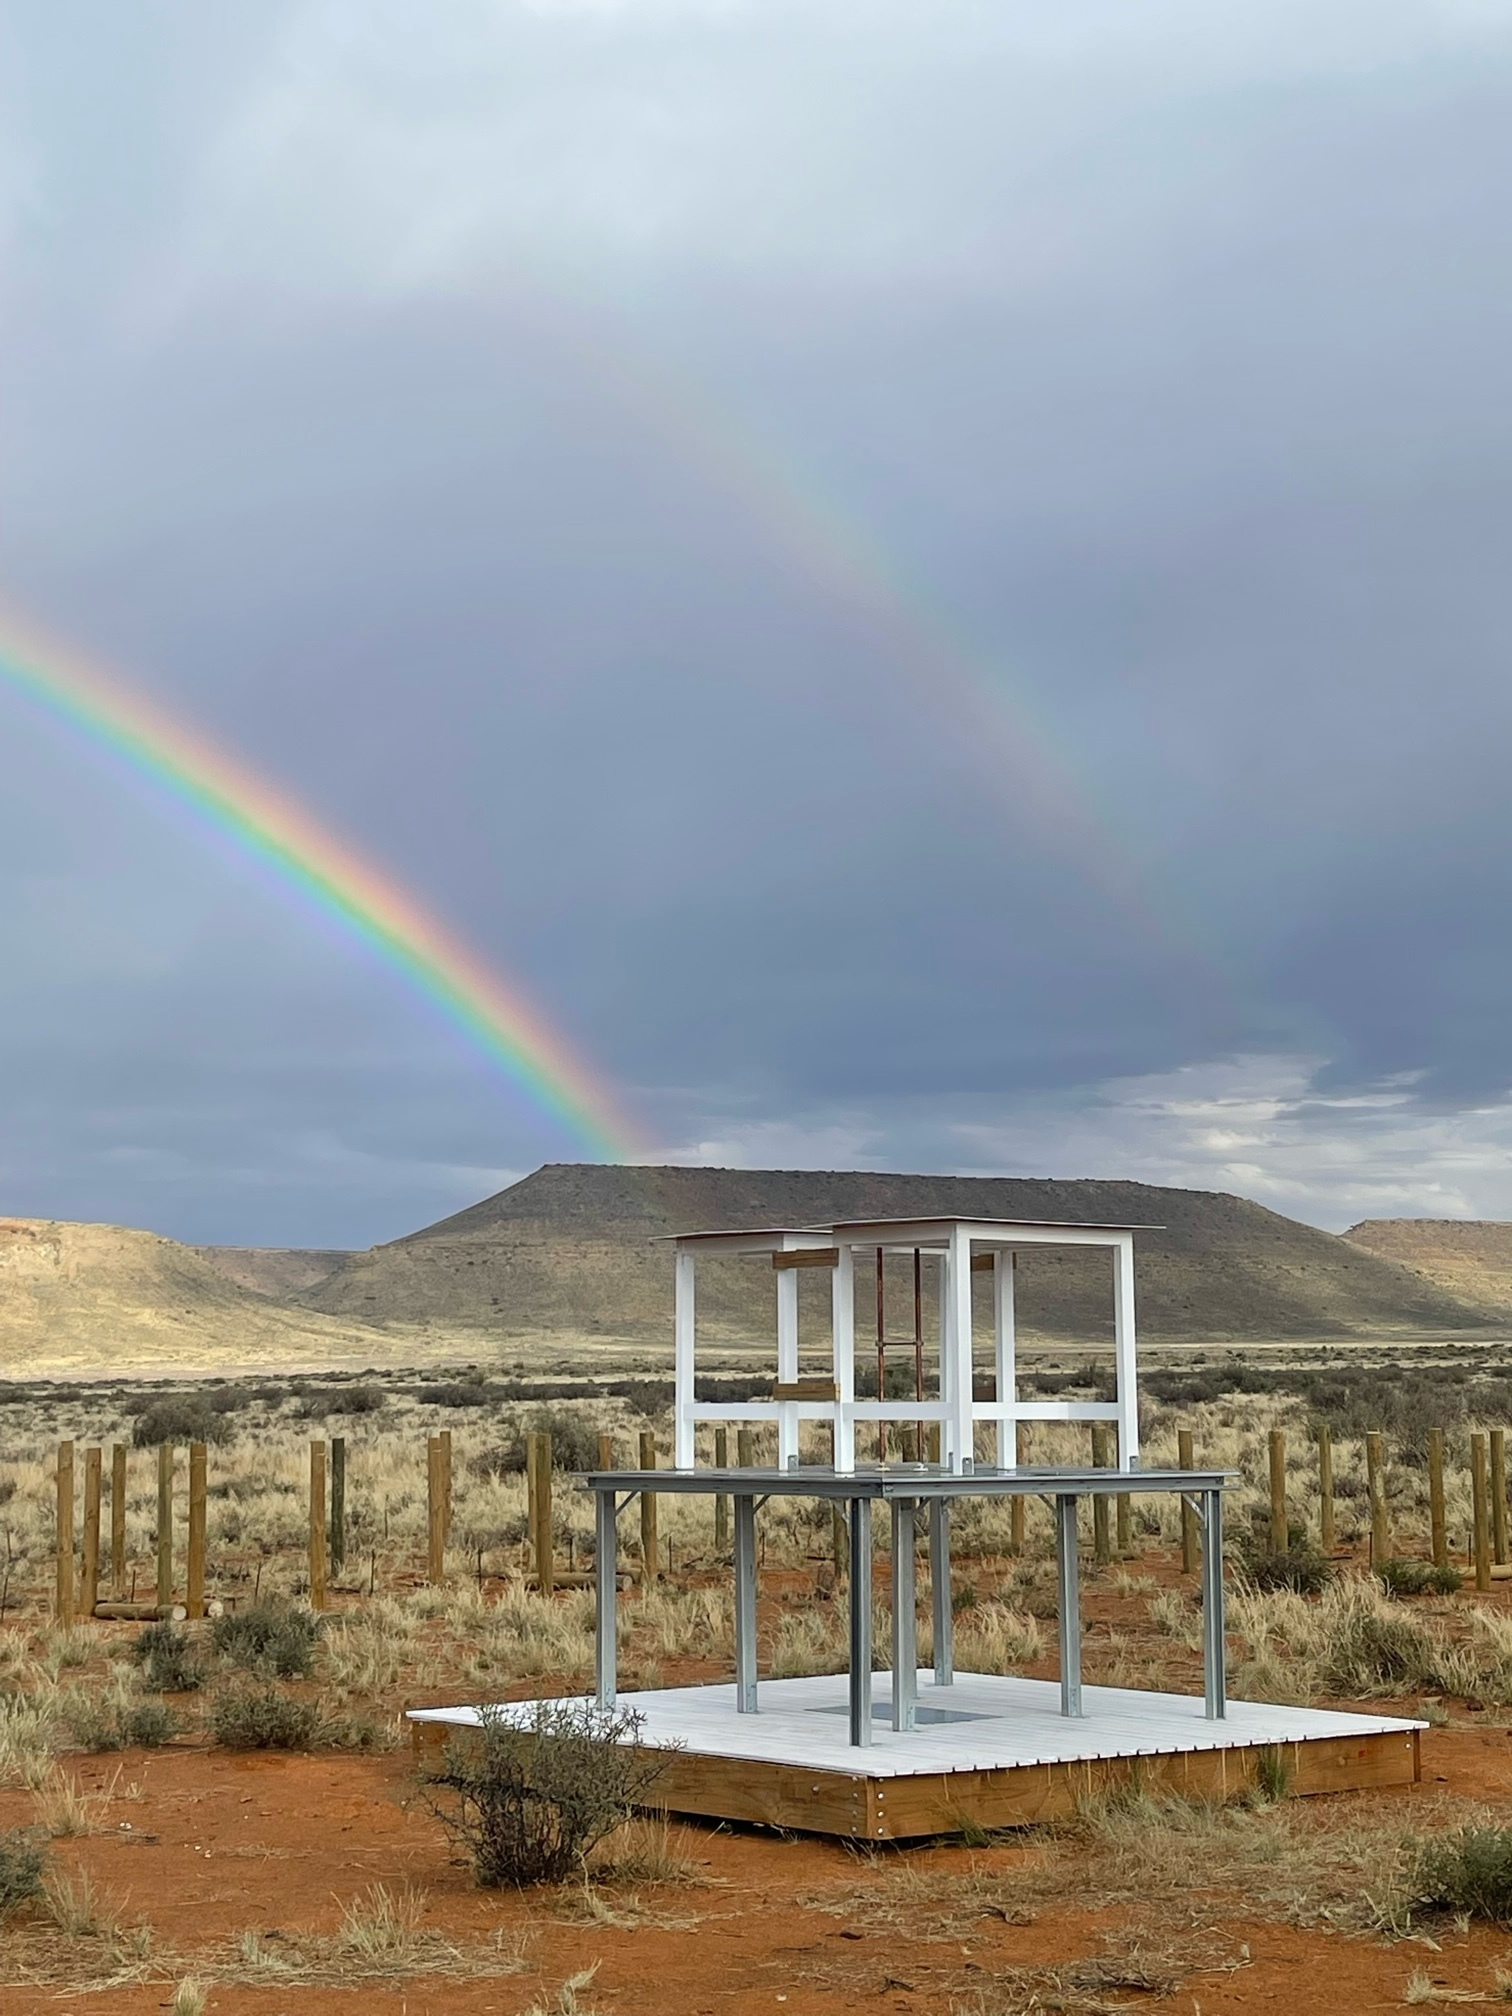
\includegraphics[height=0.3\textwidth]{figures/REACH_2.jpg}
        \end{itemize}
        \column{0.35\textwidth}
        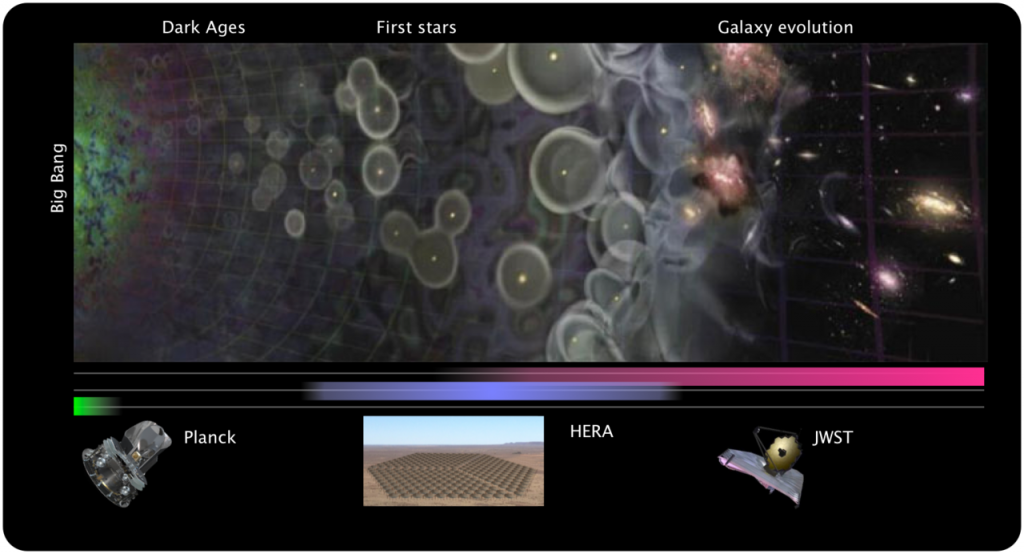
\includegraphics[width=\textwidth]{figures/21cm_1.png}
        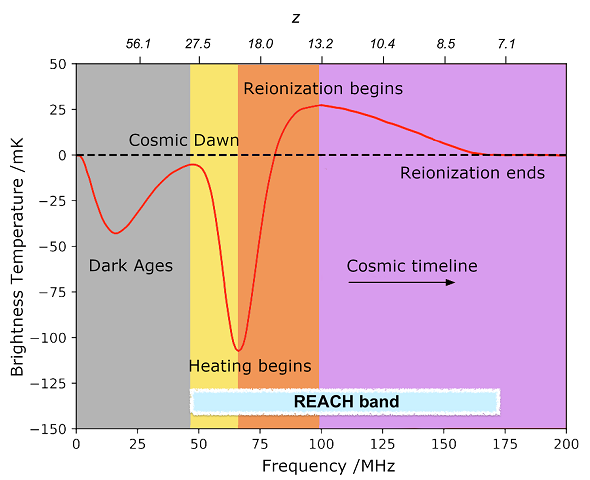
\includegraphics[width=\textwidth]{figures/21cm.png}
    \end{columns}
\end{frame}

\begin{frame}
    \frametitle{GAMBIT: combining particle physics \& cosmological data}
    \begin{columns}
        \column{0.52\textwidth}
        \begin{itemize}
            \item Multinational team of particle physicists, cosmologists and statisticians.
            \item Combine cosmological data, particle colliders, direct detection, \& neutrino detectors in a statistically principled manner~\arxiv{2205.13549}.
            \item Lead Cosmo/Dark Matter working group~\arxiv{2009.03286}.
            \item Nested sampling used for global fitting, and fine-tuning quantification~\arxiv{2101.00428}
        \end{itemize}
        \begin{center}
            
\includegraphics[width=0.5\textwidth]{figures/gambit_logo.png}
        \end{center}
        \column{0.48\textwidth}
        \vspace{-40pt}
        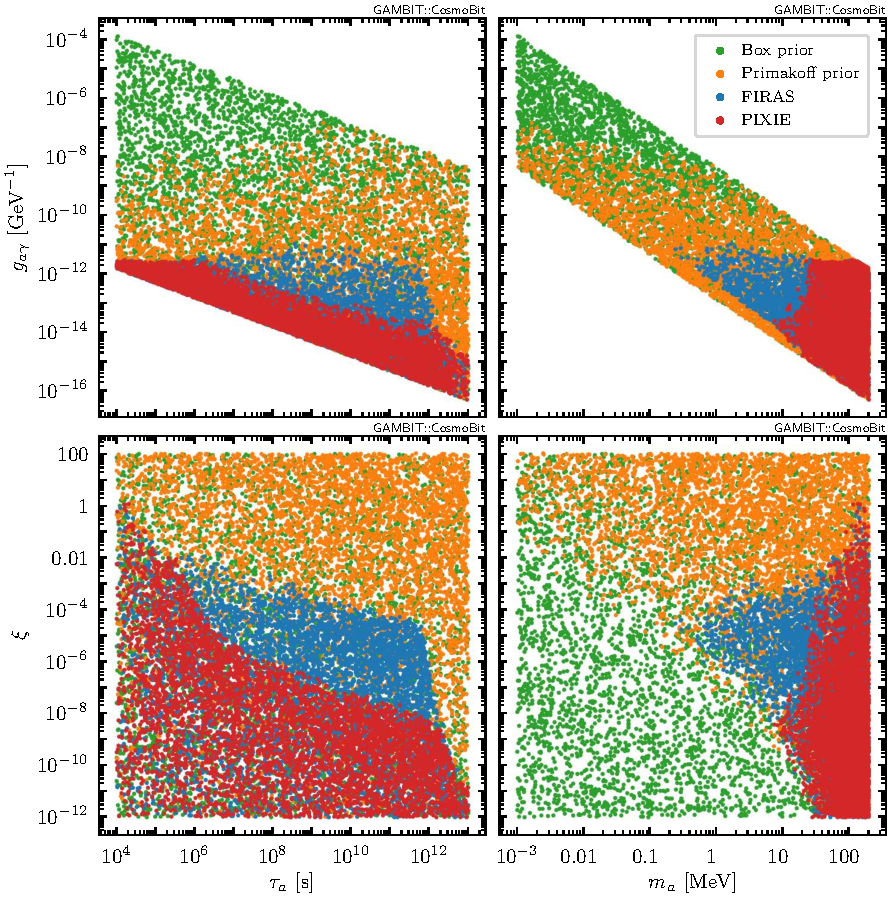
\includegraphics[width=\textwidth]{figures/ALP_2.pdf}
    \end{columns}
\end{frame}
\begin{frame}
    \frametitle{Likelihood-free inference (\& nested sampling)}
    \begin{columns}
        \column{0.5\textwidth}
        \vspace{-10pt}
        \begin{itemize}
            \item How do you do inference if you don't know the likelihood $P(D|\theta)$?
                \begin{itemize}
                    \item e.g.\ if you can simulate a disease outbreak, how can you infer a posterior on $R_0$, or select the most predictive model?
                \end{itemize}
            \item If you can forward simulate/model $\theta\to D$, then you have an implicit likelihood.
            \item LFI aims to (machine-)\emph{learn} the likelihood from carefully chosen training data $\{(\theta,D)\}$.
            \item Nested sampling has much to offer
                \begin{itemize}
                    \item truncation strategies
                    \item evidence driven compression
                    \item marginalised machine learning
                \end{itemize}
            \item In my view, LFI represents the future of inference -- in twenty years time this will be as well-used as MCMC techniques are today.
        \end{itemize}
        \column{0.5\textwidth}
        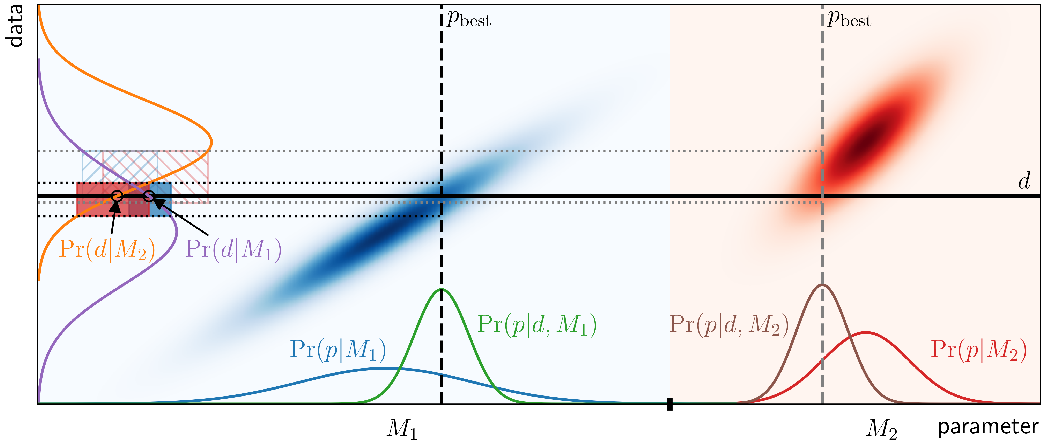
\includegraphics[width=\textwidth]{figures/noisy.pdf}
        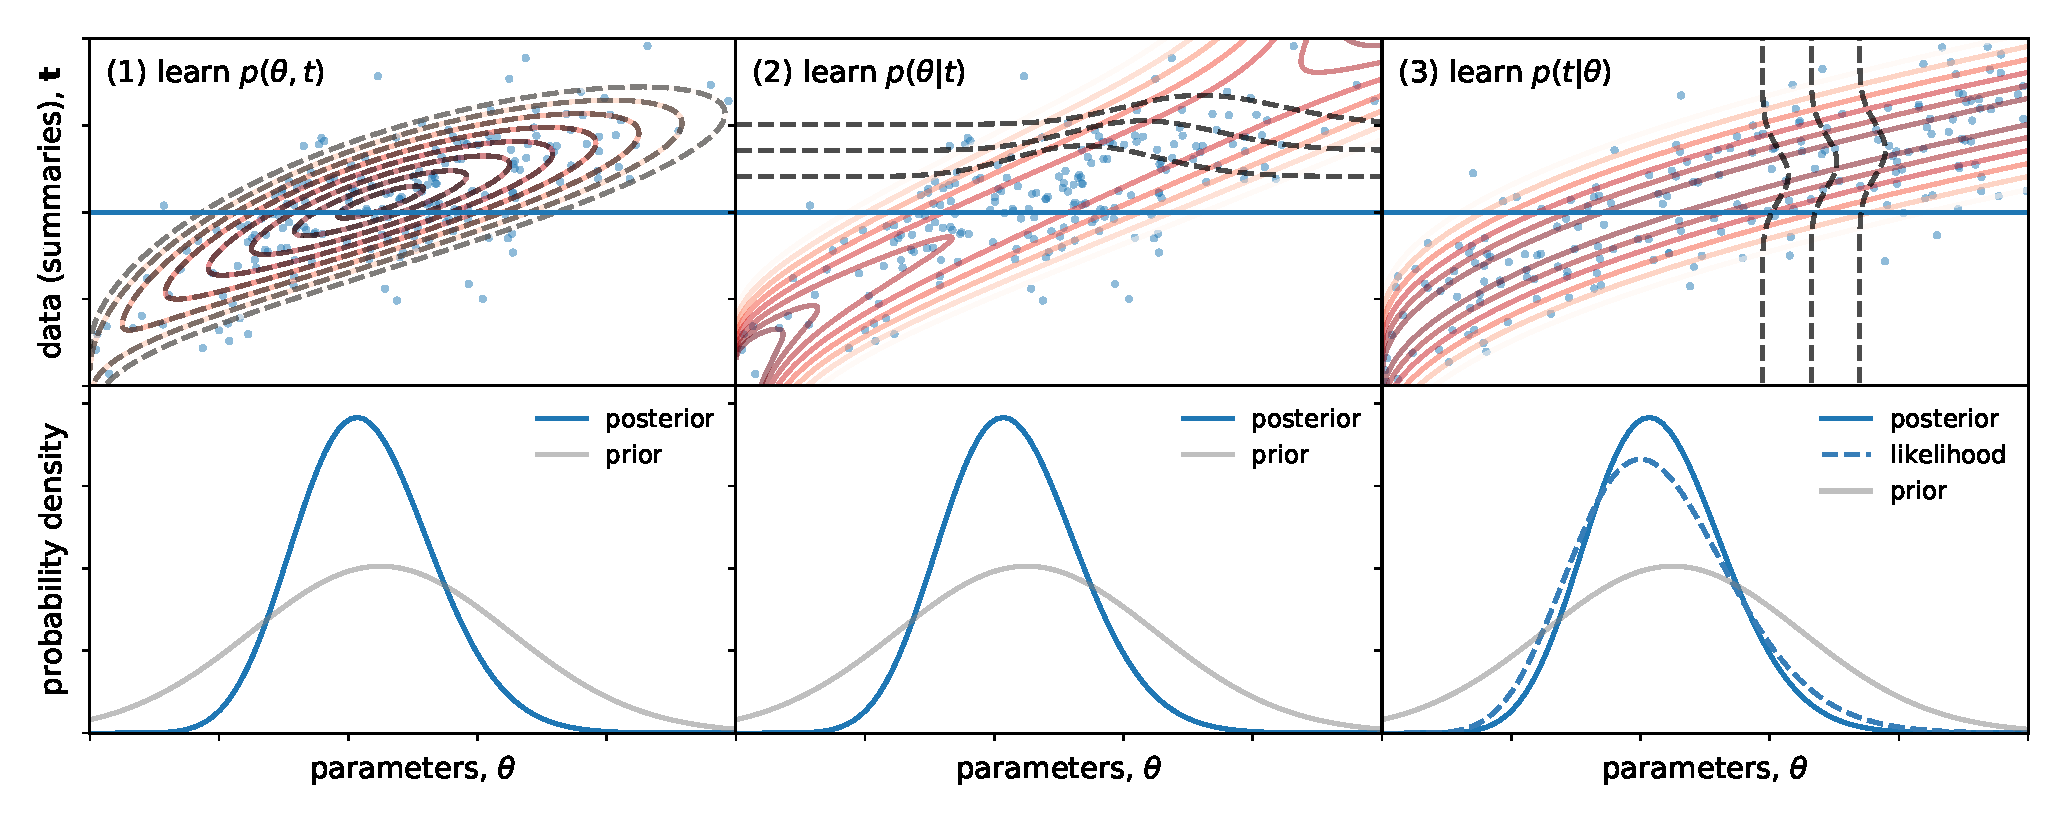
\includegraphics[width=\textwidth]{figures/three_ways_II.pdf}
    \end{columns}
\end{frame}

\begin{frame}
    \frametitle{CosmoTension}
    \framesubtitle{Resolving cosmological tensions with diverse data, novel theories and Bayesian machine learning}
    \begin{columns}
        \column{0.6\textwidth}
        \begin{itemize}
            \item ERC grant $\Rightarrow$ UKRI Frontier, commencing 2023.
            \item Funds 3 PDRAs and 4 PhDs over 5 years.
            \item Research programme centered around combining novel theories of gravity, Boltzmann solvers~\arxiv{1906.01421}, reconstruction~\arxiv{1908.00906}, nested sampling \& likelihood free inference.
            \item Aims to disentangle cosmological tensions $H_0$, $\sigma_8$, $\Omega_K$ with next-generation data analysis techniques.
        \end{itemize}
        \column{0.4\textwidth}
        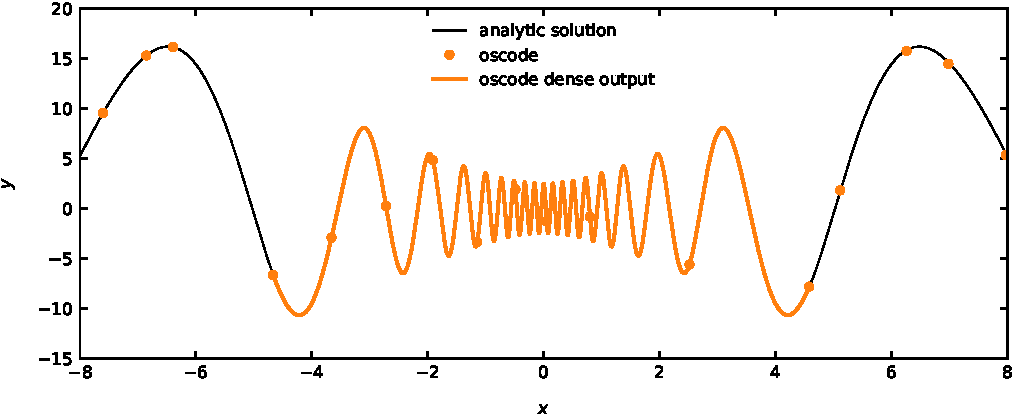
\includegraphics[width=\textwidth]{figures/denseoutput.pdf}
        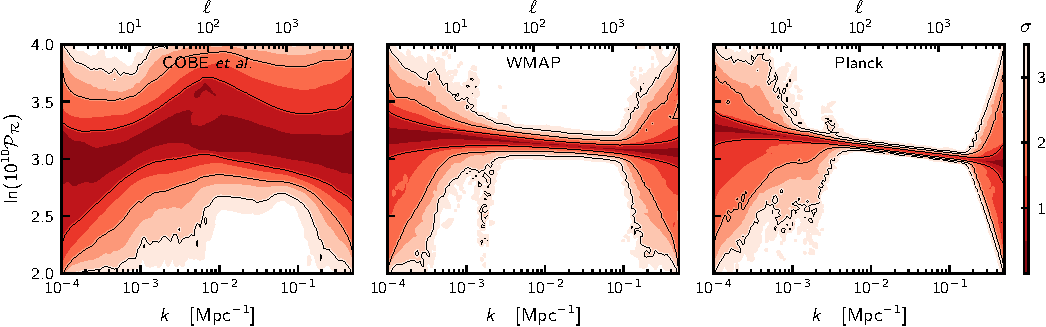
\includegraphics[width=\textwidth]{figures/pps.pdf}
        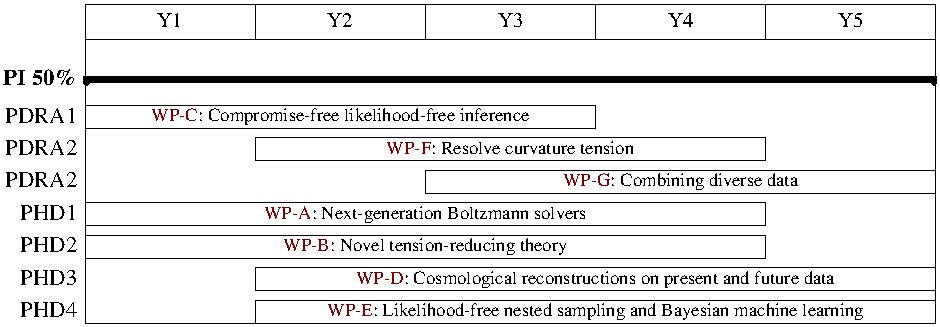
\includegraphics[width=\textwidth]{figures/gantt.pdf}
    \end{columns}
\end{frame}

\begin{frame}
    \frametitle{unimpeded: legacy suites for the next generation}
    \begin{columns}
        \column{0.5\textwidth}
        \begin{itemize}
            \item DiRAC 2020 RAC allocation of 30MCPUh
            \item Main goal: Planck Legacy Archive equivalent
            \item Parameter estimation $\to$ Model comparison
            \item MCMC $\to$ Nested sampling
            \item Planck $\to$ $\{\text{Planck}, \text{DESY1}, \text{BAO}, \ldots \}$
            \item Pairwise combinations
            \item Suite of tools for processing these 
                \begin{itemize}
                    \item \texttt{anesthetic} $2.0$
                    \item \texttt{unimpeded} $1.0$
                    \item \texttt{zenodo} archive
                    \item \texttt{margarine}
                \end{itemize}
            \item MCMC chains also available.
            \item Library of bijectors emulators for fast re-use
        \end{itemize}
        \column{0.5\textwidth}
        
\includegraphics[width=\textwidth]{logos/dirac}
        \includegraphics[width=0.5\textwidth,page=21]{figures/himmelblau}%
        \includegraphics[width=0.5\textwidth,page=15]{figures/himmelblau}
    \end{columns}
\end{frame}

\begin{frame}
    \frametitle{Summary}
    \begin{itemize}
        \item Nested sampling is a unique, multi-purpose numerical tool for:
            \begin{itemize}
                \item Numerical integration $\int f(x) dV$,
                \item Exploring/scanning/optimising \textit{a priori} unknown functions,
                \item Performing Bayesian inference: parameter estimation, model comparison \& tension quantification.
            \end{itemize}
        \item It already forms the cornerstone of many data-intensive science analyses
        \item My research innovates at the frontier of this field, and applies these techniques to a wide variety of core scientific problems working with international teams.
    \end{itemize}
\end{frame}
\appendix
\begin{frame}
    \frametitle{How does Nested Sampling compare to other approaches?}
    \begin{columns}
        \column{0.7\textwidth}
        \begin{itemize}
            \item In all cases:
                \begin{itemize}
                    \item[$+$] NS can handle multimodal functions
                    \item[$+$] NS computes evidences, partition functions and integrals
                    \item[$+$] NS is self-tuning/black-box
                \end{itemize}
        \end{itemize}
        \column{0.3\textwidth}
        Modern Nested Sampling algorithms can do this in $\sim\mathcal{O}(100s)$ dimensions
    \end{columns}
    \begin{columns}[t]
        \column{0.3\textwidth}
        \begin{block}{Optimisation}
            \begin{itemize}
                \item Gradient descent
                    \begin{itemize}
                        \item[$-$] NS cannot use gradients
                        \item[$+$] NS does not require gradients
                    \end{itemize}
                \item Genetic algorithms
                    \begin{itemize}
                        \item[$+$] NS discarded points have statistical meaning
                    \end{itemize}
            \end{itemize}
        \end{block}
        \column{0.3\textwidth}
        \begin{block}{Sampling}
            \begin{itemize}
                \item Metropolis-Hastings?
                    \begin{itemize}
                        \item[$-$] Nothing beats well-tuned customised MH
                        \item[$+$] NS is self tuning
                    \end{itemize}
                \item Hamiltonian Monte Carlo?
                    \begin{itemize}
                        \item[$-$] In millions of dimensions, HMC is king
                        \item[$+$] NS does not require gradients
                    \end{itemize}
            \end{itemize}
        \end{block}
        \column{0.3\textwidth}
        \begin{block}{Integration}
            \begin{itemize}
                \item Thermodynamic integration
                    \begin{itemize}
                        \item[$+$] protective against phase trasitions
                        \item[$+$] No annealing schedule tuning 
                    \end{itemize}
                \item Sequential Monte Carlo
                    \begin{itemize}
                        \item[$-$] SMC experts classify NS as a kind of SMC
                        \item[$+$] NS is athermal
                    \end{itemize}
            \end{itemize}
        \end{block}
    \end{columns}
\end{frame}

\begin{frame}
    \frametitle{Curvature tension: evidence for a closed universe(?)~\arxiv{1908.09139}}
    \begin{columns}
        \begin{column}{0.55\textwidth}
            \begin{itemize}
                \item If you allow $\Omega_K\ne0$, \textit{Planck} (\texttt{plikTTTEEE}) has a moderate preference for closed universes (50:1 betting odds on), $\Omega_K=-4.5\pm1.5\%$
                \item \textit{Planck}+lens+BAO strongly prefer $\Omega_K=0$.
                \item But, \textit{Planck} vs lensing is 2.5$\sigma$ in tension, and Planck vs BAO is 3$\sigma$.
                \item Reduced if $\texttt{plik}\to\texttt{camspec}$~\arxiv{2002.06892} 
                \item BAO and lensing summary assume $\Lambda$CDM.
                \item Doing this properly with BAO retains preference for closed universe (though closer to flat $\Omega_K =-0.4\pm0.2\%$)~\arxiv{2205.05892}.
                \item Present-day curvature has profound consequences for inflation~\arxiv{2205.07374}.
            \end{itemize}
        \end{column}
        \begin{column}{0.45\textwidth}
            \includegraphics<1|handout:0>[width=\textwidth]{figures/curvature_1}%
            \includegraphics<2|handout:0>[width=\textwidth]{figures/curvature_2}%
            \includegraphics<3          >[width=\textwidth]{figures/curvature_3}%
        \end{column}
    \end{columns}
\end{frame}

\end{document}
